% SHT21P kombineret temperatur- og fugtsensor

\begin{figure}[htb]
\centering
{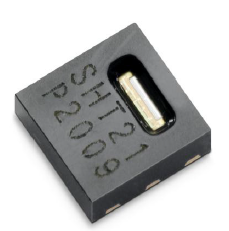
\includegraphics[width=0.25\textwidth]{filer/design/Billeder/sht21p_fysisk.png}}
\caption{Fysisk afbildning af SHT21P}
\label{lab:sht_filter}
\end{figure}

Til indsamling af temperatur- og fugtdata for golfhuller anvendes den kombineret temperatur og fugtsensor SHT21P. Denne er valgt ud fra at der således ikke behøves en sensor for hver af de to målinger, dermed sparres der et komponent. SHT21P sender en PWM ud som midles til en DC-spænding med et 2. ordens lavpasfilter. Denne spændingen sendes ind i en A/D-convertor i PSoCen hvor denne behandles i en funktion, for så at returnere en temperatur eller fugt. Et select ben på SHT21P angiver hvorvidt denne måler temp. eller fugt. SCL HIGH(1) giver fugt output, SCL LOW(0) giver temperatur output.

\subsection{Foranliggende filter}
\begin{figure}[htb]
\centering
{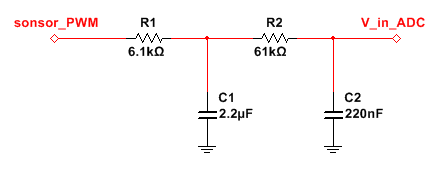
\includegraphics[width=0.75\textwidth]{filer/design/Billeder/sht21p_filter_pic.png}}
\caption{Multisim tegninger af 2. ordens filter}
\label{lab:sht_filter_pic}
\end{figure}

2. ordens filteret er sammensat af to lavpasfiltre. Det første filter, bestående af R1 og C1 bestemmer knækfrekvensen. Det efterfølgende filter, R2 og C2, er valgt som en faktor 10 af R1 og C1 hvilket vil resultere i et 2. ordens filter, men samtidig vil de to ikke påvirke hinanden og kan derfor forbindes direkte uden en buffer. 

Filterets knækfrekvens ($f_c$) er designet ud fra frekvensen på PWM signalet. Denne er opgivet til 120 Hz i databladet. Ved at designe filteret med en $f_c$ der ligger væsentligt under 120 Hz, vil der opnås en stor dæmpning, således at signalet tilnærmer sig en fast DC-spænding svarende til middelværdien af PWM. PWMen oscillerer i området VSS-VDD. Sensoren er forsynet med 3,3 VDC og VSS er forbundet til GND, hvilket giver en PWM i området 0-3,3 V. DC-spændingen efter filteret er testet ved 10 \% dutycycle og 90 \% dutycycle hvilket gav henholdsvis 211 mV og 2610 mV efter filteret. Ligningerne for udregning af fugt og temp., er opgivet som en funktion af PWMen, er begge lineære og der kan derfor regnes med et step i volt på grader celsius. Funktionerne herfor er opgivet i databladet for SHT21P. 
På figur \ref{lab:sht_plot_mable} kan det ses at kurven for fugtighed går fra -6 \% til 120 \%, denne er dog kun defineret ved 0 til 100 \%. 

% PLOT FRA MAPLE HER!
\begin{figure}[htb]
\centering
{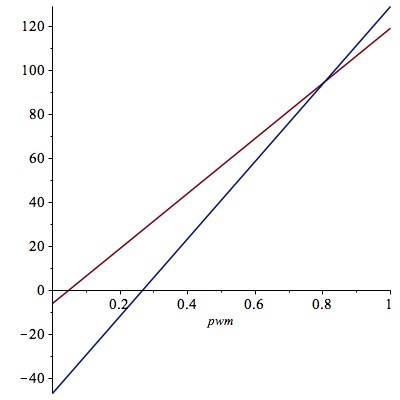
\includegraphics[width=0.75\textwidth]{filer/design/Billeder/sht_plot_maple.png}}
\caption{Plot af fugt(rød kurve) og temperatur(blå kurve) som funktion af pwm}
\label{lab:sht_plot_mable}
\end{figure}

\subsection{Præcisions- og støjhåndtering}
%Beskriv step i mV pr. grader celsius her. Magter det ikke nu /Jakob

Ved 10\% duty cycle og 90\% duty cycle vil DC-spændingen give henholdsvis 33 mV og 2970 mV $<=> \Delta V = 2970$ og en temperatur differens gående fra -29 ... 111 ${^{\circ}}$C $<=> \Delta T = 140 {^{\circ}}$C. Da denne er en lineær funktion kan der beregnes et step:

\begin{equation}
step = \frac{2970}{140} = 21 \frac{mV}{^{\circ}C}
\end{equation}


\begin{equation}
f_c = \frac{1}{2 \pi * R1 * C1} = \frac{1}{2 \pi * 6,1*10^3  * 2,2*10^{-6}} = 12 Hz\pm5 \%
\end{equation}

Da komponenternes værdi har en afvigelse på $\pm$5 \%.
$f_c$ ligger således en dekade under 120 Hz og da filteret er designet som et 2. ordens filter, vil det dæmpe 40 dB pr. dekade. Amplituden vil da være dæmpet 100 gange og tilbage er den tilnærmede DC-værdi. 

\begin{equation}
Gain = 20 * \log_{10}(x) <=> 40 dB = 20 * \log_ {10}(x) <=> x = 100
\end{equation} 
Da det er en dæmpning der er tale om, vil gain være lig med -40 dB hvilket vil give en x-værdi på 0,01 som er det samme som 100 gange dæmpning.

Grundet at værdien kun er tilnærmet skyldes at der stadig vil være oscillation tilbage fra PWMen og det antages at denne svarer til 33 mV. Der vil altså være en usikkerhed i DC-værdien svarende til 1,6 $^{\circ}$C alene fra filteret. De 33 mV er en ideel antagelse ud fra filteret, men nøjagtigheden herfor kan ikke garanteres og der laves derfor en antagelse.

Dette kan løses i softwaren ved evt. at tage et antal samples og så midle de værdier der er målt med simple gennemsnitsberegning. 

\begin{equation}
V_{inADC_{avg}} = \frac{V_{in1} + V_{in2} + .. V_{inN}}{N}
\end{equation} 
\textit{hvor N = antal samples}

En anden støjfaktor der er værd at tage hensyn til er filterets belastning af udgangen på sensoren. Denne kan have indflydelse på området hvori PWM'en går højt og lavt. Det kan altså ikke med sikkerhed siges at signalet vil gå fra 0 V til 3,3 V, men kan have et offset og en evt. dæmpning. Denne problematik kan løses ved indsættelse af en OpAmp, forbundet som en komparator, med kendt spændingsforsyning i det ønsket område, lige før filteret. Denne vil sørge for, at signalet kommer til at ligge i det valgte område. En OpAmp fra HC14 familien ville kunne klare denne opgave. 

\begin{figure}[htb]
\centering
{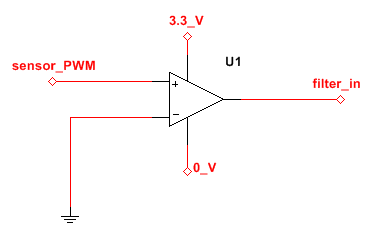
\includegraphics[width=0.75\textwidth]{filer/design/Billeder/sht_opamp.png}}
\caption{OpAmp til udbedring af evt. støj forårsaget af lavpasfilter}
\label{lab:sht_opamp}
\end{figure}
